\let\negmedspace\undefined
\let\negthickspace\undefined
\documentclass[journal]{IEEEtran}
\usepackage[a5paper, margin=10mm, onecolumn]{geometry}
%\usepackage{lmodern} % Ensure lmodern is loaded for pdflatex
\usepackage{tfrupee} % Include tfrupee package

\setlength{\headheight}{1cm} % Set the height of the header box
\setlength{\headsep}{0mm}     % Set the distance between the header box and the top of the text

\usepackage{gvv-book}
\usepackage{gvv}
\usepackage{cite}
\usepackage{amsmath,amssymb,amsfonts,amsthm}
\usepackage{algorithmic}
\usepackage{graphicx}
\usepackage{textcomp}
\usepackage{xcolor}
\usepackage{txfonts}
\usepackage{listings}
\usepackage{enumitem}
\usepackage{mathtools}
\usepackage{gensymb}
\usepackage{comment}
\usepackage[breaklinks=true]{hyperref}
\usepackage{tkz-euclide} 
\usepackage{listings}
% \usepackage{gvv}                                        
\def\inputGnumericTable{}                                 
\usepackage[latin1]{inputenc}                                
\usepackage{color}                                            
\usepackage{array}                                            
\usepackage{longtable}                                       
\usepackage{calc}                                             
\usepackage{multirow}                                         
\usepackage{hhline}                                           
\usepackage{ifthen}                                           
\usepackage{lscape}
\begin{document}

\bibliographystyle{IEEEtran}
\vspace{3cm}

\title{CHAPTER - 3\\Constructions}
\author{EE24BTECH11061 - Rohith Sai}
% \maketitle
% \newpage
% \bigskip
{\let\newpage\relax\maketitle}

\renewcommand{\thefigure}{\theenumi}
\renewcommand{\thetable}{\theenumi}
\setlength{\intextsep}{10pt} % Space between text and floats

\numberwithin{figure}{enumi}
\renewcommand{\thetable}{\theenumi}

\section{3.2 Triangle}
\begin{enumerate}
\item [3.2.8] Draw a triangle $ABC$ in which $AB = 5cm$, $BC = 6cm$ and $\angle ABC = 60\degree$.\\
\textbf{Solution:}
\begin{table}[h!]
      \centering
      \begin{tabular}[12pt]{ |c| c|}
    \hline
    \textbf{Variable} & \textbf{Description}\\ 
    \hline
    $x\brak{0}$ & First term of the AP \\
    \hline 
    $d$ & Common difference of the AP\\
    \hline
    $y\brak{n}$ & Sum of $n+1$ terms of the AP\\
    \hline
    $x\brak{n}$ & General term\\
    \hline   
    \end{tabular}
      \caption{}
\end{table}\\
Let $\vec{k} = \vec{b} + \vec{c}$,\\
Using cosine rule, we can find the length of $AC$, i.e., $\vec{b}$:
\begin{align}
    b^2 = a^2 + c^2 - 2ac\cos{B}\\
\end{align}
On solving, we get $\vec{b}$ as:
\begin{align}
    \vec{b} = \sqrt{31}cm
\end{align}
Therefore, we get:
\begin{align}
    \vec{k} = \sqrt{31} + 5 cm
\end{align}
From the above table, we get the following triangle:
\begin{figure}
    \centering
    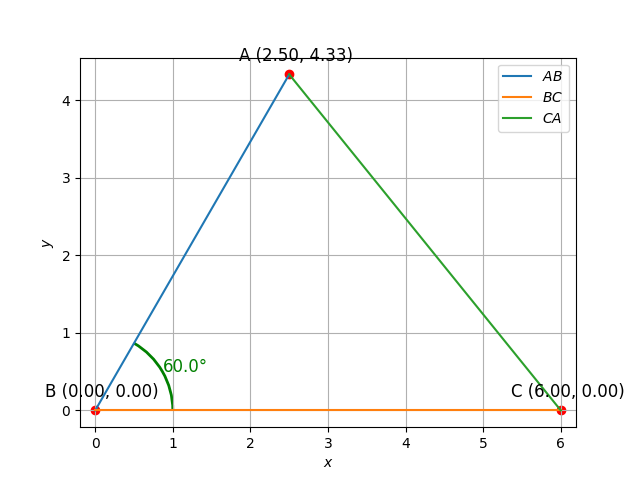
\includegraphics[width=10cm]{figs/figure.png}
    \caption{}
    \label{fig:enter-label}
\end{figure}
\end{enumerate}
\end{document}